\documentclass{ximera}

\begin{document}

\begin{question}
  Find 
  \[
  \displaystyle \lim_{x\to0} \frac{x+1}{x^2+3x}
  \]
  \begin{solution}
    \begin{hint}
      This function is \underline{not} continuous everywhere, but both the numerator and denominator are continuous everywhere as functions. Thus, if the limit of $\frac{x+1}{x^2+3x}$ as $x\to a$ does not exist, then the denominator $x^2+3x$ must be zero at $a$.
    \end{hint}
     \begin{hint}
    Take a look at the graph of the function
    \begin{center}
     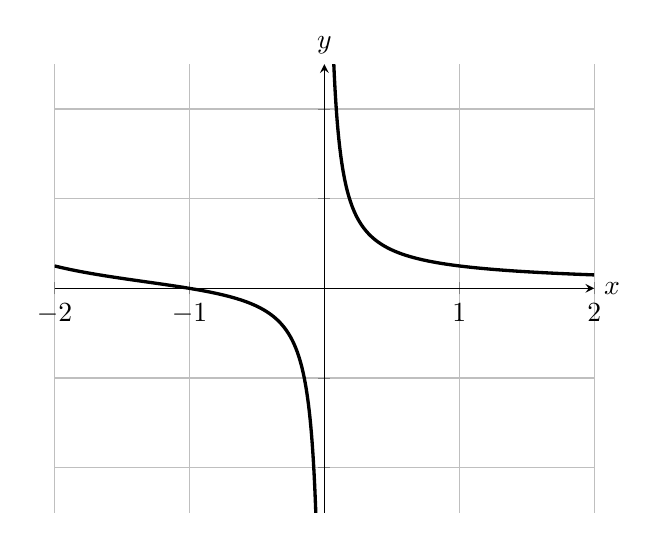
\begin{tikzpicture}
	\begin{axis}
	[ymin=-5,ymax=5, axis lines=center,xlabel=$x$,ylabel=$y$,every axis y 
	label/.style={at=(current axis.above origin),anchor=south},every axis x label/.style={at=(current axis.right of origin),anchor=west},
	domain=-2:2,
	yticklabels={},
	ymajorgrids=true,
	grid = major
	]
	\addplot[domain=-2:-1/100,very thick,smooth,samples=500]
	{(\x+1)/(\x^2+3*\x)};
	\addplot[domain=1/100:2,very thick,smooth,samples=500]
	{(\x+1)/(\x^2+3*\x)};
	\end{axis}
       \end{tikzpicture}      
      \end{center}
    \end{hint}
    \begin{hint}
     Evaluating $\lim\limits_{x\to0^{-}}\frac{x+1}{x^2+3x}$ we see that it tends to $-\infty$. This follows because, for $-3\le x\le0$, $x^2+3x\le0$ (after all, $x^2+3x=0$ when $x=-3$), and for $-1\le x\le0$, $x+1\ge0$; hence, for $-1\le x<0$, $\frac{x+1}{x^2+3x}\le0$. Moreover, $x^2+3x$ tends to $0$ as $x\to{0}$ and $x+1$ tends to $1$ as $x\to{0}$. These two observations tell us that  $\lim\limits_{x\to0^{-}}\frac{x+1}{x^2+3x}$ tends to $-\infty$. This is sufficient to know the answer, regardless of whether or not the limit approaching $0$ from the right is also $-\infty$ or not.
    \end{hint}
    \answer{\text{Limit does not exist}}.
  \end{solution}
\end{question}

\end{document}